\documentclass[
	12pt,				
	openright,			
	oneside,			
	a4paper,			
	english,			
	brazilian			
	]{abntex2}

% ---
% Pacotes básicos 
% ---
\usepackage{lmodern}			
\usepackage[T1]{fontenc}		
\usepackage[utf8]{inputenc}		
\usepackage{indentfirst}		
\usepackage{color}				
\usepackage{graphicx}			
\usepackage{microtype} 			
\usepackage{listings}			
\usepackage{pdfpages}			
\usepackage{tikz}				% para diagramas de blocos
\usetikzlibrary{shapes,arrows,positioning,calc}
% ---

% Compatibilidade memoir vs abntex2cite
% ---
\renewcommand{\tt}{\normalfont\ttfamily} % Corrige erro de comando \tt obsoleto

% ---
% Configurações de listings para MicroPython
% ---
\definecolor{codegreen}{rgb}{0,0.6,0}
\definecolor{codegray}{rgb}{0.5,0.5,0.5}
\definecolor{codepurple}{rgb}{0.58,0,0.82}
\definecolor{backcolour}{rgb}{0.95,0.95,0.92}

\lstset{
    language=Python,
    backgroundcolor=\color{backcolour},   
    commentstyle=\color{codegreen},
    keywordstyle=\color{magenta},
    numberstyle=\tiny\color{codegray},
    stringstyle=\color{codepurple},
    basicstyle=\ttfamily\footnotesize,
    breakatwhitespace=false,         
    breaklines=true,                 
    captionpos=b,                    
    keepspaces=true,                 
    numbers=left,                    
    numbersep=5pt,                  
    showspaces=false,                
    showstringspaces=false,
    showtabs=false,                  
    tabsize=2,
    extendedchars=true,
    inputencoding=utf8,
    literate={á}{{\'a}}1 {ã}{{\~a}}1 {â}{{\^a}}1 {à}{{\`a}}1 {Á}{{\'A}}1 {Ã}{{\~A}}1 {Â}{{\^A}}1 {À}{{\`A}}1
             {é}{{\'e}}1 {ê}{{\^e}}1 {É}{{\'E}}1 {Ê}{{\^E}}1
             {í}{{\'i}}1 {Í}{{\'I}}1
             {ó}{{\'o}}1 {õ}{{\~o}}1 {ô}{{\^o}}1 {Ó}{{\'O}}1 {Õ}{{\~O}}1 {Ô}{{\^O}}1
             {ú}{{\'u}}1 {Ú}{{\'U}}1
             {ç}{{\c{c}}}1 {Ç}{{\c{C}}}1 {—}{{---}}1 {→}{{$\rightarrow$}}1 {°}{{$^\circ$}}1
}

% ---
% Pacotes de citações
% ---
\usepackage[brazilian,hyperpageref]{backref}
\usepackage[alf,abnt-emphasize=bf]{abntex2cite}	% Citações padrão ABNT

% --- 
% CONFIGURAÇÕES DE PACOTES
% --- 
\renewcommand{\backrefpagesname}{Citado na(s) página(s):~}
\renewcommand{\backref}{}
\renewcommand*{\backrefalt}[4]{
	\ifcase #1 
		Nenhuma citação no texto.
	\or
		Citado na página #2.
	\else
		Citado na página #2.
	\fi}

% ---
% Informações de dados para CAPA e CONTRA CAPA
% ---
\titulo{Projeto Semestral: Carro de Bombeiro Teleoprado}
\autor{Felipe Fazio da Costa, RA: 23.00055-4 \\ João Gabriel Fioruci Roberto, RA: 23.00617-0 \\ Gabriel Rodrigues Marques, RA: 23.00578-5 \\ Fábio Sadao Sato, RA: 22.00984-0}
\local{Brasil}
\data{2026}
\instituicao{%
  Centro Universitário Instituto Mauá de Tecnologia
  \par
  Engenharia de Computação / Eletrônica
  \par
  Disciplina: EEN251 --- Projeto de Sistemas Embarcados}
\tipotrabalho{Relatório Técnico}
\preambulo{Relatório técnico apresentado como requisito parcial para aprovação na disciplina EEN251 --- Projeto Integrador de Sistemas Embarcados do curso de Engenharia.}

% ---
% Configurações de aparência do PDF final
\definecolor{blue}{RGB}{41,5,195}

\hypersetup{
		pdftitle={Projeto Semestral: Carro de Bombeiro Teleoprado}, 
		pdfauthor={Felipe Fazio da Costa, João Gabriel Fioruci Roberto, Gabriel Rodrigues Marques, Fábio Sadao Sato},
    	pdfsubject={Relatório técnico de Projeto Integrador},
	    pdfcreator={LaTeX with abntex2},
		pdfkeywords={abnt}{latex}{pico}{nrf24l01}{carro de bombeiro}, 
		colorlinks=true,       		
    	linkcolor=blue,          	
    	citecolor=blue,        		
    	filecolor=magenta,      		
		urlcolor=blue,
		bookmarksdepth=4
}

% --- 
% Espaçamentos entre linhas e parágrafos 
% --- 
\setlength{\parindent}{1.3cm}
\setlength{\parskip}{0.2cm}  

\makeindex

% ----
\begin{document}
\selectlanguage{brazilian}
\frenchspacing 

% ----------------------------------------------------------
\imprimircapa
\imprimirfolhaderosto

\begin{resumo}
 Este relatório descreve o desenvolvimento de um protótipo de carro de bombeiro teleoprado utilizando microcontroladores Raspberry Pi Pico e comunicação via rádio frequência (NRF24L01). O sistema integra tração 4WD, sistema de combate a incêndio por bomba d'água e monitoramento de nível de reservatório. Foram aplicados conceitos de sistemas embarcados, comunicação sem fio e controle de periféricos via PWM. Os resultados demonstram a eficácia da plataforma RP2040 em aplicações de controle em tempo real e teleoperação robusta.

 \vspace{\onelineskip}
    
 \noindent
 \textbf{Palavras-chave}: Raspberry Pi Pico. NRF24L01. MicroPython. Carro de Bombeiro. Sistemas Embarcados.
\end{resumo}

\begin{resumo}[Abstract]
 \begin{otherlanguage*}{english}
   This report describes the development of a teleoperated fire truck prototype using Raspberry Pi Pico microcontrollers and radio frequency communication (NRF24L01). The system integrates 4WD traction, a water pump fire suppression system, and reservoir level monitoring. Concepts of embedded systems, wireless communication, and peripheral control via PWM were applied. The results demonstrate the effectiveness of the RP2040 platform in real-time control applications and robust teleoperation.

   \vspace{\onelineskip}
 
   \noindent
   \textbf{Keywords}: Raspberry Pi Pico. NRF24L01. MicroPython. Fire Truck. Embedded Systems.
 \end{otherlanguage*}
\end{resumo}

\pdfbookmark[0]{\contentsname}{toc}
\tableofcontents*
\cleardoublepage

% ----------------------------------------------------------
\textual

\chapter{Introdução}

O projeto semestral da disciplina EEN251 --- Projeto Integrador de Sistemas Embarcados propõe o desenvolvimento de um sistema embarcado completo, integrando hardware e software. O tema escolhido foi um carro de bombeiro teleoprado, que combina mobilidade, atuação remota e sensoriamento.

O uso de veículos teleoperados é comum em situações de risco, como o combate a incêndios, onde a segurança humana é prioridade. O protótipo desenvolvido busca simular essas funcionalidades em escala reduzida.

\section{Objetivos}

O objetivo geral deste trabalho é projetar e construir um veículo robótico controlado remotamente via radiofrequência, capaz de realizar manobras de locomoção e acionamento de uma bomba d'água, com monitoramento de status em tempo real.

Como objetivos específicos, destacam-se:
\begin{itemize}
    \item Implementação de comunicação bidirecional robusta entre controle e veículo;
    \item Controle de tração diferencial (tank drive) para quatro motores;
    \item Sistema de alerta de nível de água com indicadores visuais e sonoros;
    \item Desenvolvimento de firmware em MicroPython para a plataforma Raspberry Pi Pico.
\end{itemize}

\chapter{Desenvolvimento do Projeto}

O desenvolvimento foi dividido em três frentes principais: hardware, software e integração de sistemas.

\section{Arquitetura e Diagramas de Blocos}

A Figura \ref{fig:diagrama_geral} apresenta a visão sistêmica do projeto, destacando a separação entre as unidades de controle e de atuação no veículo.

\begin{figure}[htb]
    \centering
    \caption{Diagrama de Blocos do Sistema Completo}
    \label{fig:diagrama_geral}
    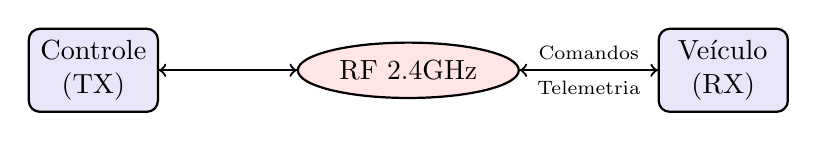
\begin{tikzpicture}[node distance=4cm, auto, thick,
        block/.style={rectangle, draw, fill=blue!10, text width=4em, text centered, rounded corners, minimum height=3em},
        cloud/.style={draw, ellipse, fill=red!10, node distance=4cm, minimum height=2em}]
        
        \node [block] (tx) {Controle (TX)};
        \node [cloud, right of=tx] (rf) {RF 2.4GHz};
        \node [block, right of=rf] (rx) {Veículo (RX)};
        
        \path [draw, ->] (tx) -- (rf);
        \path [draw, ->, bend left] (rf) -- node [above, font=\scriptsize] {Comandos} (rx);
        \path [draw, ->, bend left] (rx) -- node [below, font=\scriptsize] {Telemetria} (rf);
        \path [draw, ->] (rf) -- (tx);
    \end{tikzpicture}
    \legend{Fonte: Os autores (2026)}
\end{figure}

\subsection{Subsistema Transmissor (Controle)}

O controle remoto (Figura \ref{fig:diagrama_tx}) processa as entradas do joystick e botões através do Raspberry Pi Pico, transmitindo-as via NRF24L01.

\begin{figure}[htb]
    \centering
    \caption{Fluxo de Dados do Transmissor}
    \label{fig:diagrama_tx}
    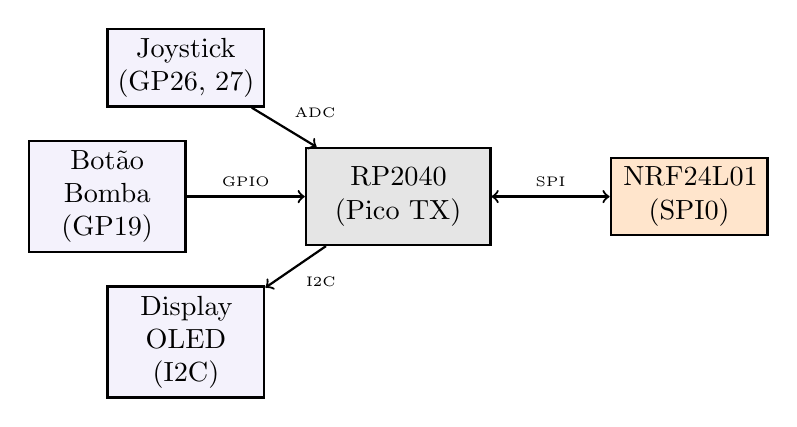
\begin{tikzpicture}[node distance=1.5cm, auto, thick,
        cpu/.style={rectangle, draw, fill=gray!20, text width=6em, text centered, minimum height=3.5em},
        inout/.style={rectangle, draw, fill=blue!5, text width=5em, text centered, minimum height=2em}]
        
        \node [cpu] (pico) {RP2040 (Pico TX)};
        \node [inout, above left=0.5cm and 0.5cm of pico] (joy) {Joystick (GP26, 27)};
        \node [inout, left=of pico] (btn) {Botão Bomba (GP19)};
        \node [inout, below left=0.5cm and 0.5cm of pico] (oled) {Display OLED (I2C)};
        \node [inout, right=of pico, fill=orange!20] (nrf) {NRF24L01 (SPI0)};
        
        \draw [->] (joy) -- node [font=\tiny] {ADC} (pico);
        \draw [->] (btn) -- node [font=\tiny] {GPIO} (pico);
        \draw [->] (pico) -- node [font=\tiny] {I2C} (oled);
        \draw [<->] (pico) -- node [font=\tiny] {SPI} (nrf);
    \end{tikzpicture}
    \legend{Fonte: Os autores (2026)}
\end{figure}

\subsection{Subsistema Receptor (Veículo)}

O receptor (Figura \ref{fig:diagrama_rx}) traduz os sinais RF em comandos de potência para os motores e gerencia os sensores de campo.

\begin{figure}[htb]
    \centering
    \caption{Fluxo de Atuação do Receptor}
    \label{fig:diagrama_rx}
    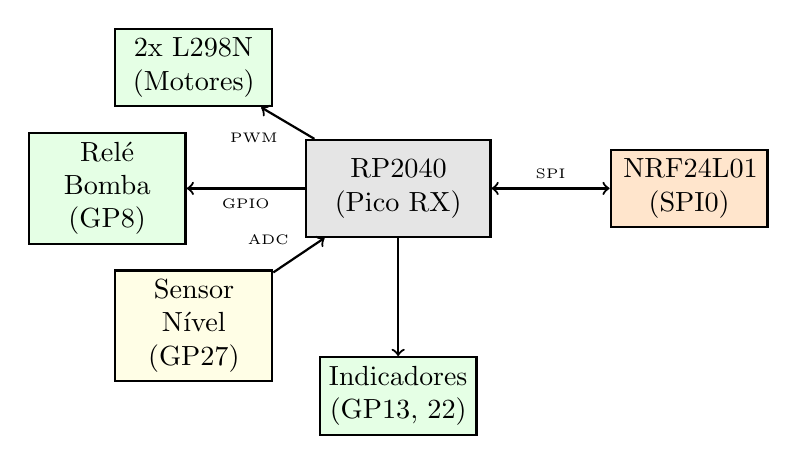
\begin{tikzpicture}[node distance=1.5cm, auto, thick,
        cpu/.style={rectangle, draw, fill=gray!20, text width=6em, text centered, minimum height=3.5em},
        act/.style={rectangle, draw, fill=green!10, text width=5em, text centered, minimum height=2em},
        sens/.style={rectangle, draw, fill=yellow!10, text width=5em, text centered, minimum height=2em}]
        
        \node [cpu] (pico) {RP2040 (Pico RX)};
        \node [act, above left=0.4cm and 0.4cm of pico] (l298n) {2x L298N (Motores)};
        \node [act, left=of pico] (rele) {Relé Bomba (GP8)};
        \node [sens, below left=0.4cm and 0.4cm of pico] (umid) {Sensor Nível (GP27)};
        \node [act, right=of pico, fill=orange!20] (nrf) {NRF24L01 (SPI0)};
        \node [act, below=of pico] (leds) {Indicadores (GP13, 22)};
        
        \draw [->] (pico) -- node [font=\tiny] {PWM} (l298n);
        \draw [->] (pico) -- node [font=\tiny] {GPIO} (rele);
        \draw [->] (umid) -- node [font=\tiny] {ADC} (pico);
        \draw [<->] (pico) -- node [font=\tiny] {SPI} (nrf);
        \draw [->] (pico) -- (leds);
    \end{tikzpicture}
    \legend{Fonte: Os autores (2026)}
\end{figure}

\section{Arquitetura de Hardware}

O sistema é composto por dois nós principais: o Transmissor (Controle) e o Receptor (Veículo). Ambos utilizam o microcontrolador RP2040 \cite{rp2040:datasheet}, presente na placa Raspberry Pi Pico \cite{pico:datasheet}.

\subsection{Transmissor (Controle)}

O controle remoto utiliza um joystick analógico para comandos de direção e botões para acionamento da bomba. Um display OLED SSD1306 foi integrado para fornecer feedback visual ao operador.

\subsection{Receptor (Veículo)}

O veículo possui um chassi 4WD acionado por motores DC. O controle de potência é realizado por drivers L298N \cite{l298n:datasheet}. O sistema possui uma mini bomba submersa acionada por relé.

\section{Comunicação RF (NRF24L01)}

A comunicação utiliza o módulo NRF24L01 \cite{nrf24l01:product} operando em 2.4 GHz. Foi adotado o protocolo Enhanced ShockBurst. Todo o desenvolvimento do rádio foi baseado na biblioteca \cite{nrf24l01:library}.

\section{Software e Firmware}

Todo o código foi desenvolvido em MicroPython \cite{micropython:docs}. O firmware gerencia a recepção de pacotes e o controle de periféricos.

\subsection{Lógica de Movimentação (Tank Drive)}

\begin{lstlisting}[caption={Algoritmo de Tank Drive em MicroPython}]
def drive(x, y):
    motor_esq = max(-100, min(100, y + x))
    motor_dir = max(-100, min(100, y - x))
    set_motor(motor_esq, motor_dir)
\end{lstlisting}

\subsection{Segurança e Failsafe}

\begin{lstlisting}[caption={Logica de Watchdog}]
if time.ticks_diff(time.ticks_ms(), ultimo_sinal) > 500:
    parar()        # Desliga motores por seguranca
\end{lstlisting}

\section{Modelagem 3D e Estrutura Física}

A estrutura física foi projetada em CAD. A Figura \ref{fig:modelagem3d} apresenta a renderização do veículo.

\begin{figure}[htb]
	\caption{\label{fig:modelagem3d}Modelagem 3D do Carro de Bombeiro}
	\begin{center}
	    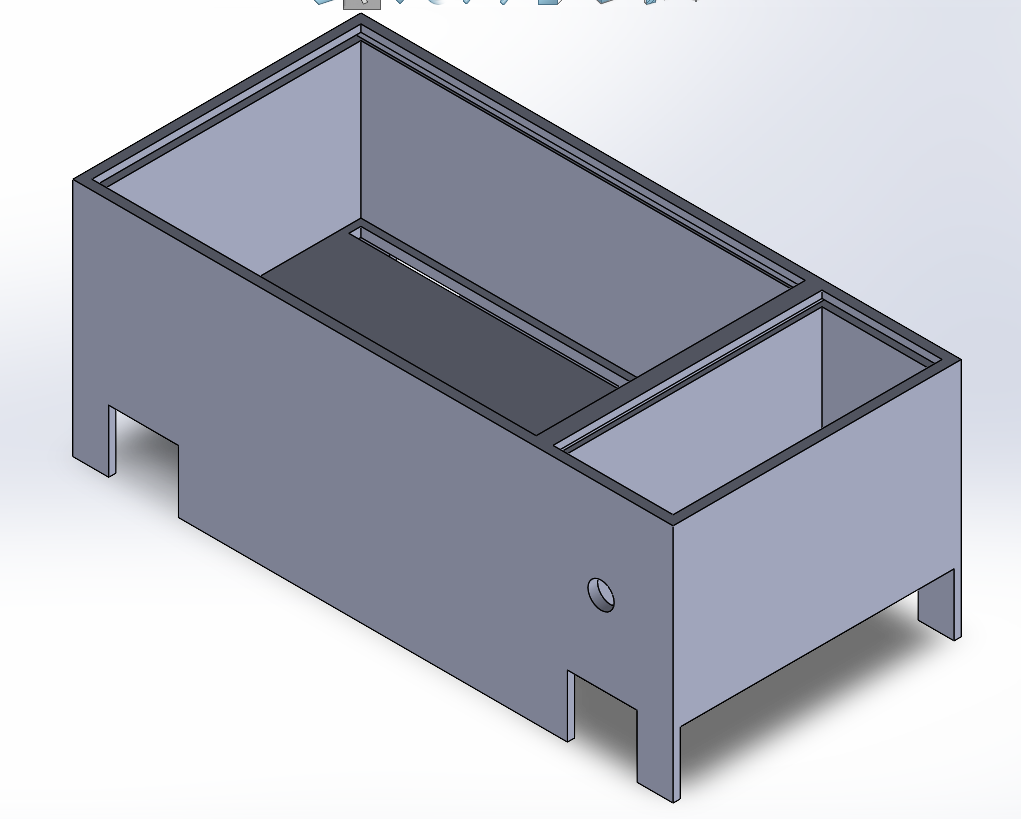
\includegraphics[width=0.7\textwidth]{../../Modelos 3D Solid/Carro.png}
	  \end{center}
	\legend{Fonte: Os autores (2026)}
\end{figure}

\begin{figure}[htb]
    \centering
    \begin{minipage}{0.45\textwidth}
        \centering
        \caption{Base do Controle}
        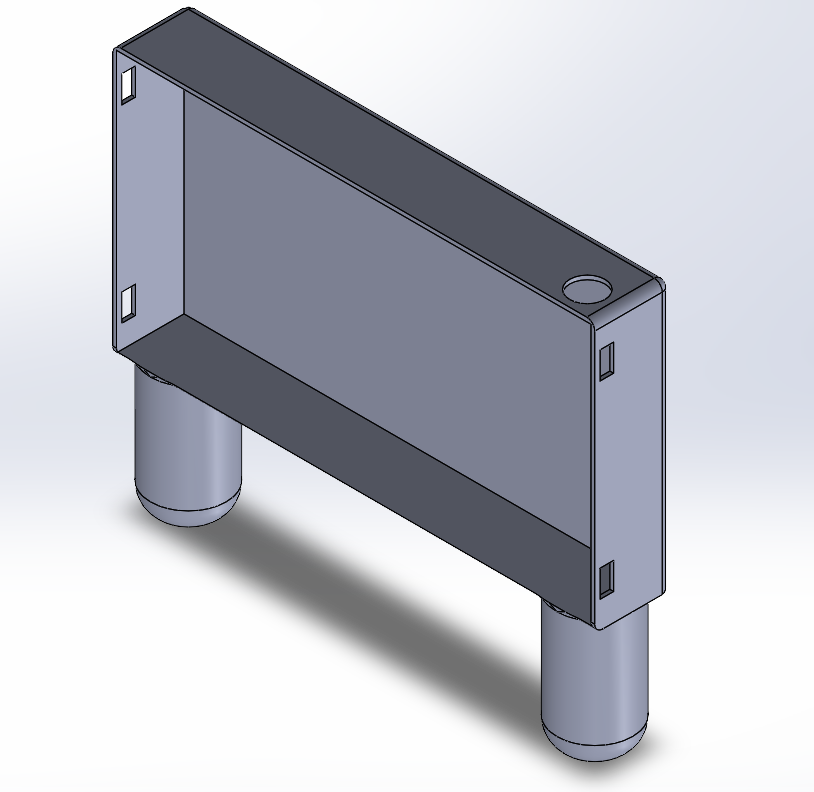
\includegraphics[width=\textwidth]{../../Modelos 3D Solid/Controle Base.png}
        \label{fig:controle_base}
    \end{minipage}
    \hfill
    \begin{minipage}{0.45\textwidth}
        \centering
        \caption{Tampa do Controle}
        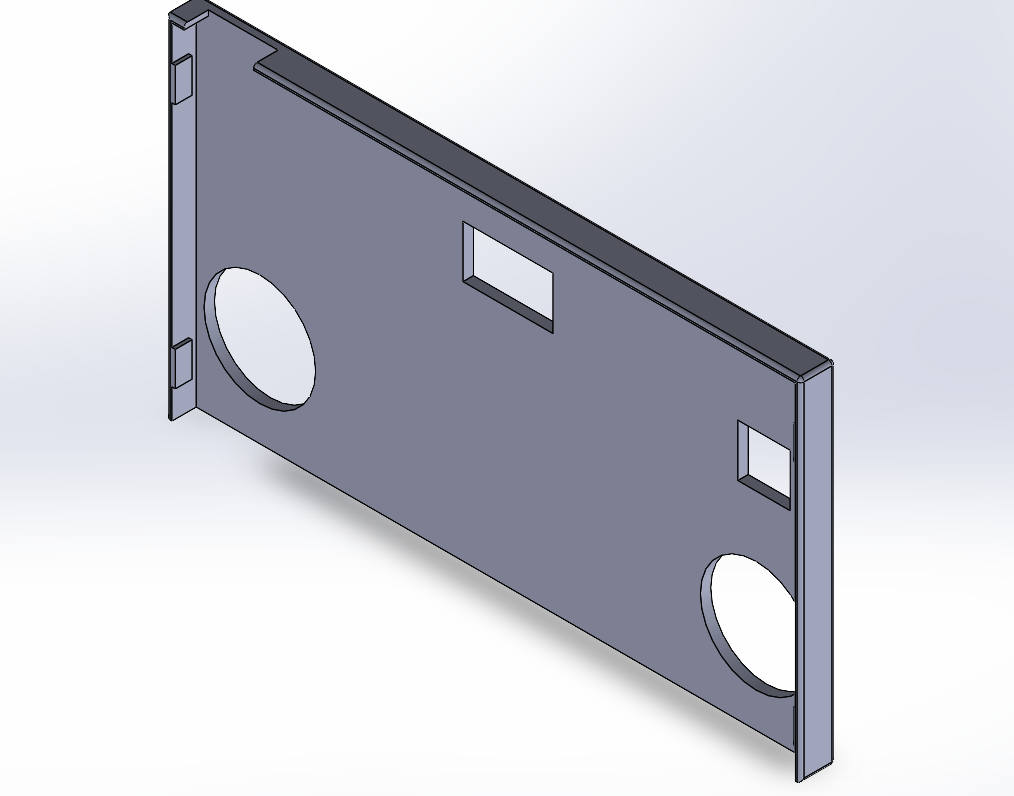
\includegraphics[width=\textwidth]{../../Modelos 3D Solid/Controle Tampa.png}
        \label{fig:controle_tampa}
    \end{minipage}
    \legend{Fonte: Os autores (2026)}
\end{figure}

\section{Esquemas Elétricos e PCB}

A Figura \ref{fig:pcb3d} ilustra a visualização 3D da PCB do carro, enquanto a Figura \ref{fig:pcb3d_controle} apresenta a visualização 3D da PCB do controle.

\begin{figure}[htb]
	\caption{\label{fig:pcb3d}Visualização 3D da PCB do Carro}
	\begin{center}
	    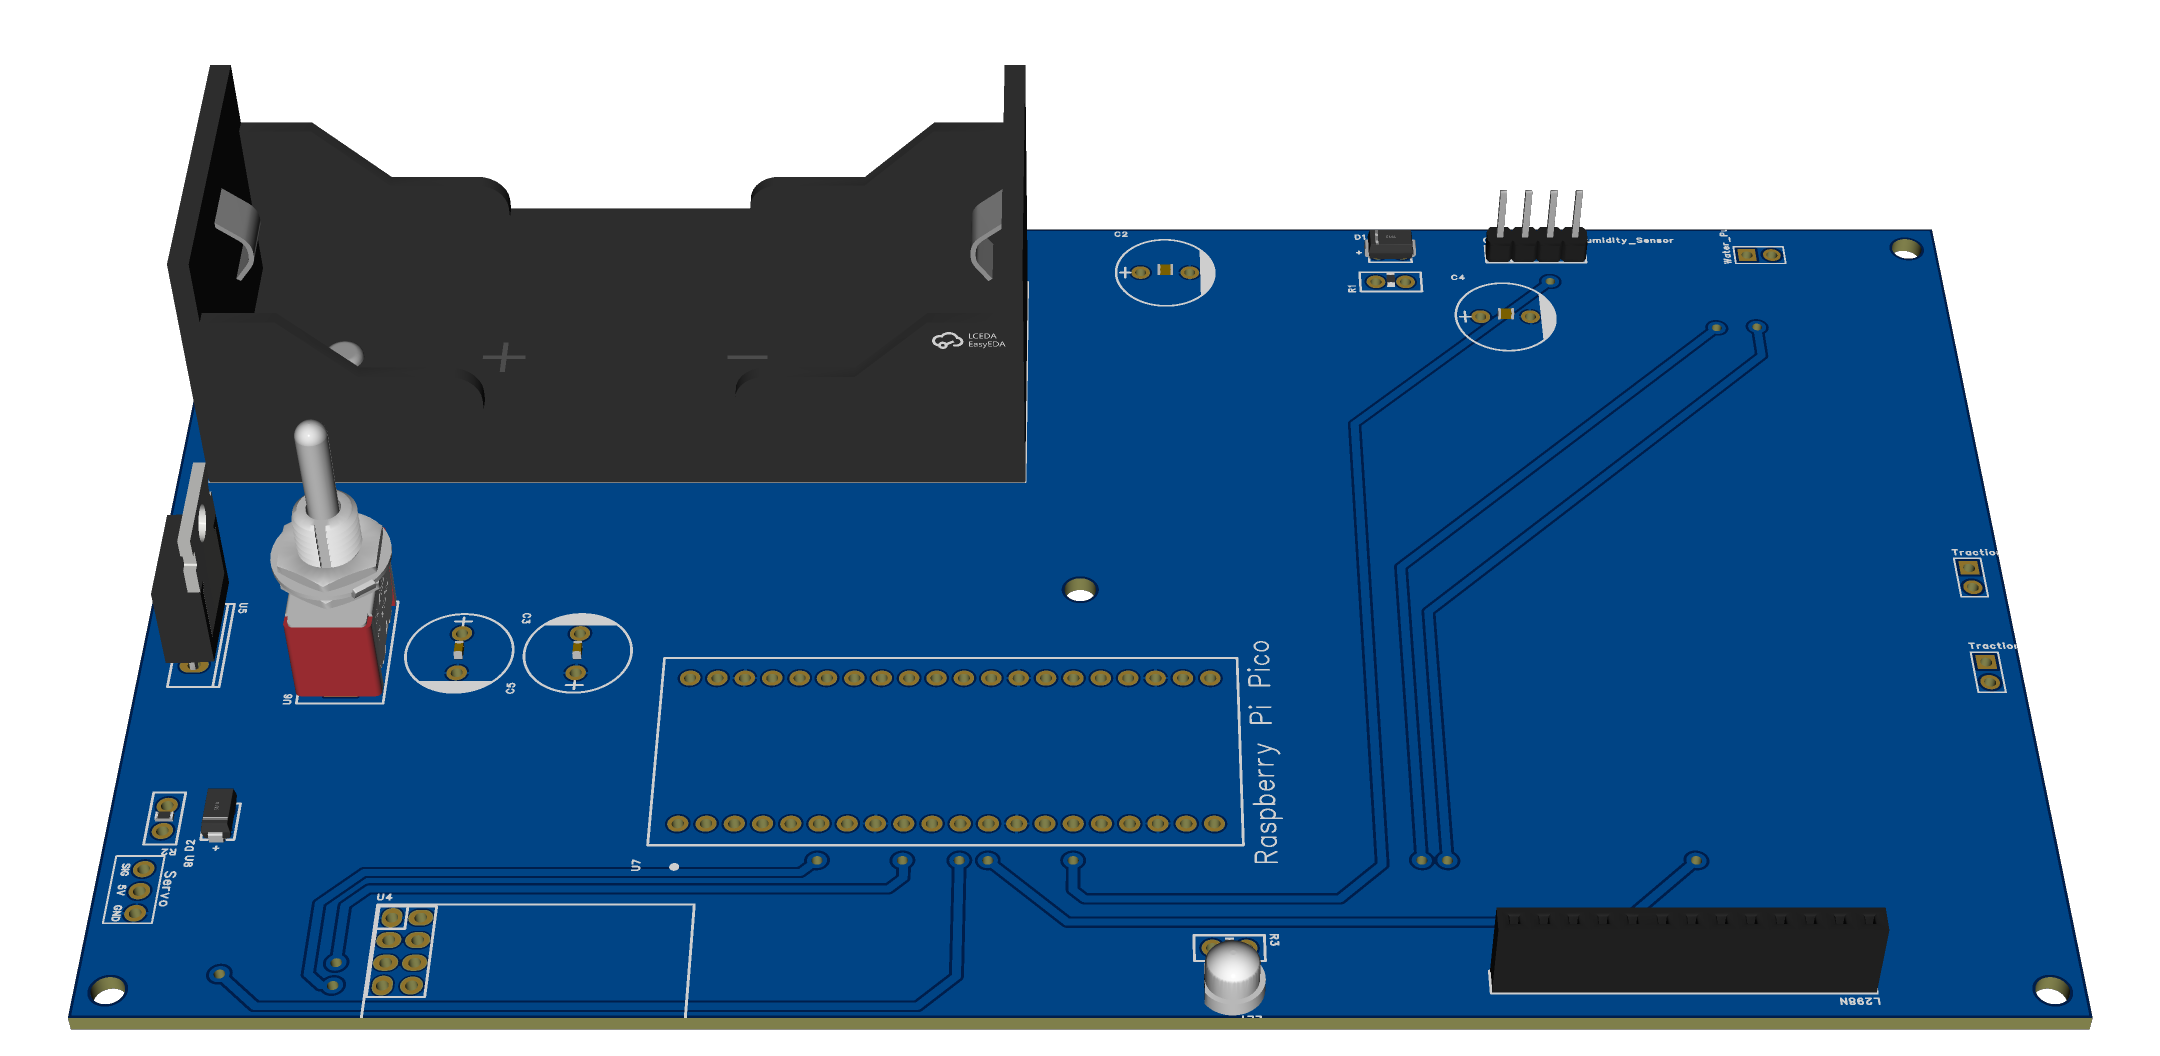
\includegraphics[width=0.7\textwidth]{../../Esquemas elétricos/Carro/Esquema PCB 3D.png}
	  \end{center}
	\legend{Fonte: Os autores (2026)}
\end{figure}

\begin{figure}[htb]
	\caption{\label{fig:pcb3d_controle}Visualização 3D da PCB do Controle}
	\begin{center}
	    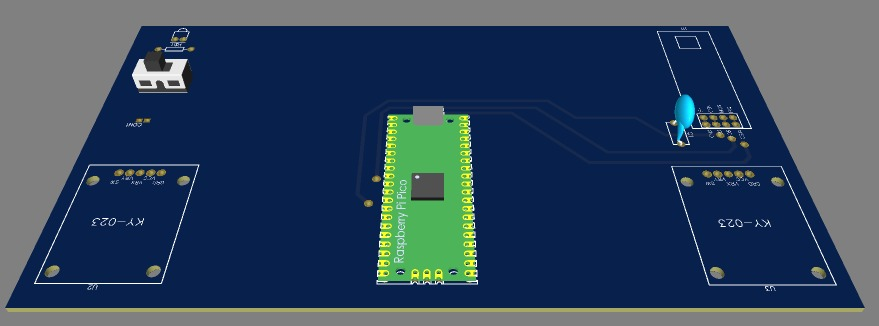
\includegraphics[width=0.7\textwidth]{../../Esquemas elétricos/Controle/Esquema PCB 3D.jpeg}
	  \end{center}
	\legend{Fonte: Os autores (2026)}
\end{figure}


\chapter{Conclusão}

O projeto atingiu os objetivos. A integração NRF24L01/RP2040 permitiu uma teleoperação robusta e segura.

\postextual

% ----------------------------------------------------------
% Referências bibliográficas
% ----------------------------------------------------------
\bibliography{referencias}

% ---
% Apêndices
% ---
\begin{apendicesenv}
\partapendices

\chapter{Código Fonte do Receptor}
\lstinputlisting[language=Python]{../../src/carro de bombeiro/carro.py}

\chapter{Código Fonte do Transmissor}
\lstinputlisting[language=Python]{../../src/controle/controle.py}

\end{apendicesenv}

% ---
% Anexos
% ---
\begin{anexosenv}
\partanexos

\chapter{Esquema Elétrico do Carro}
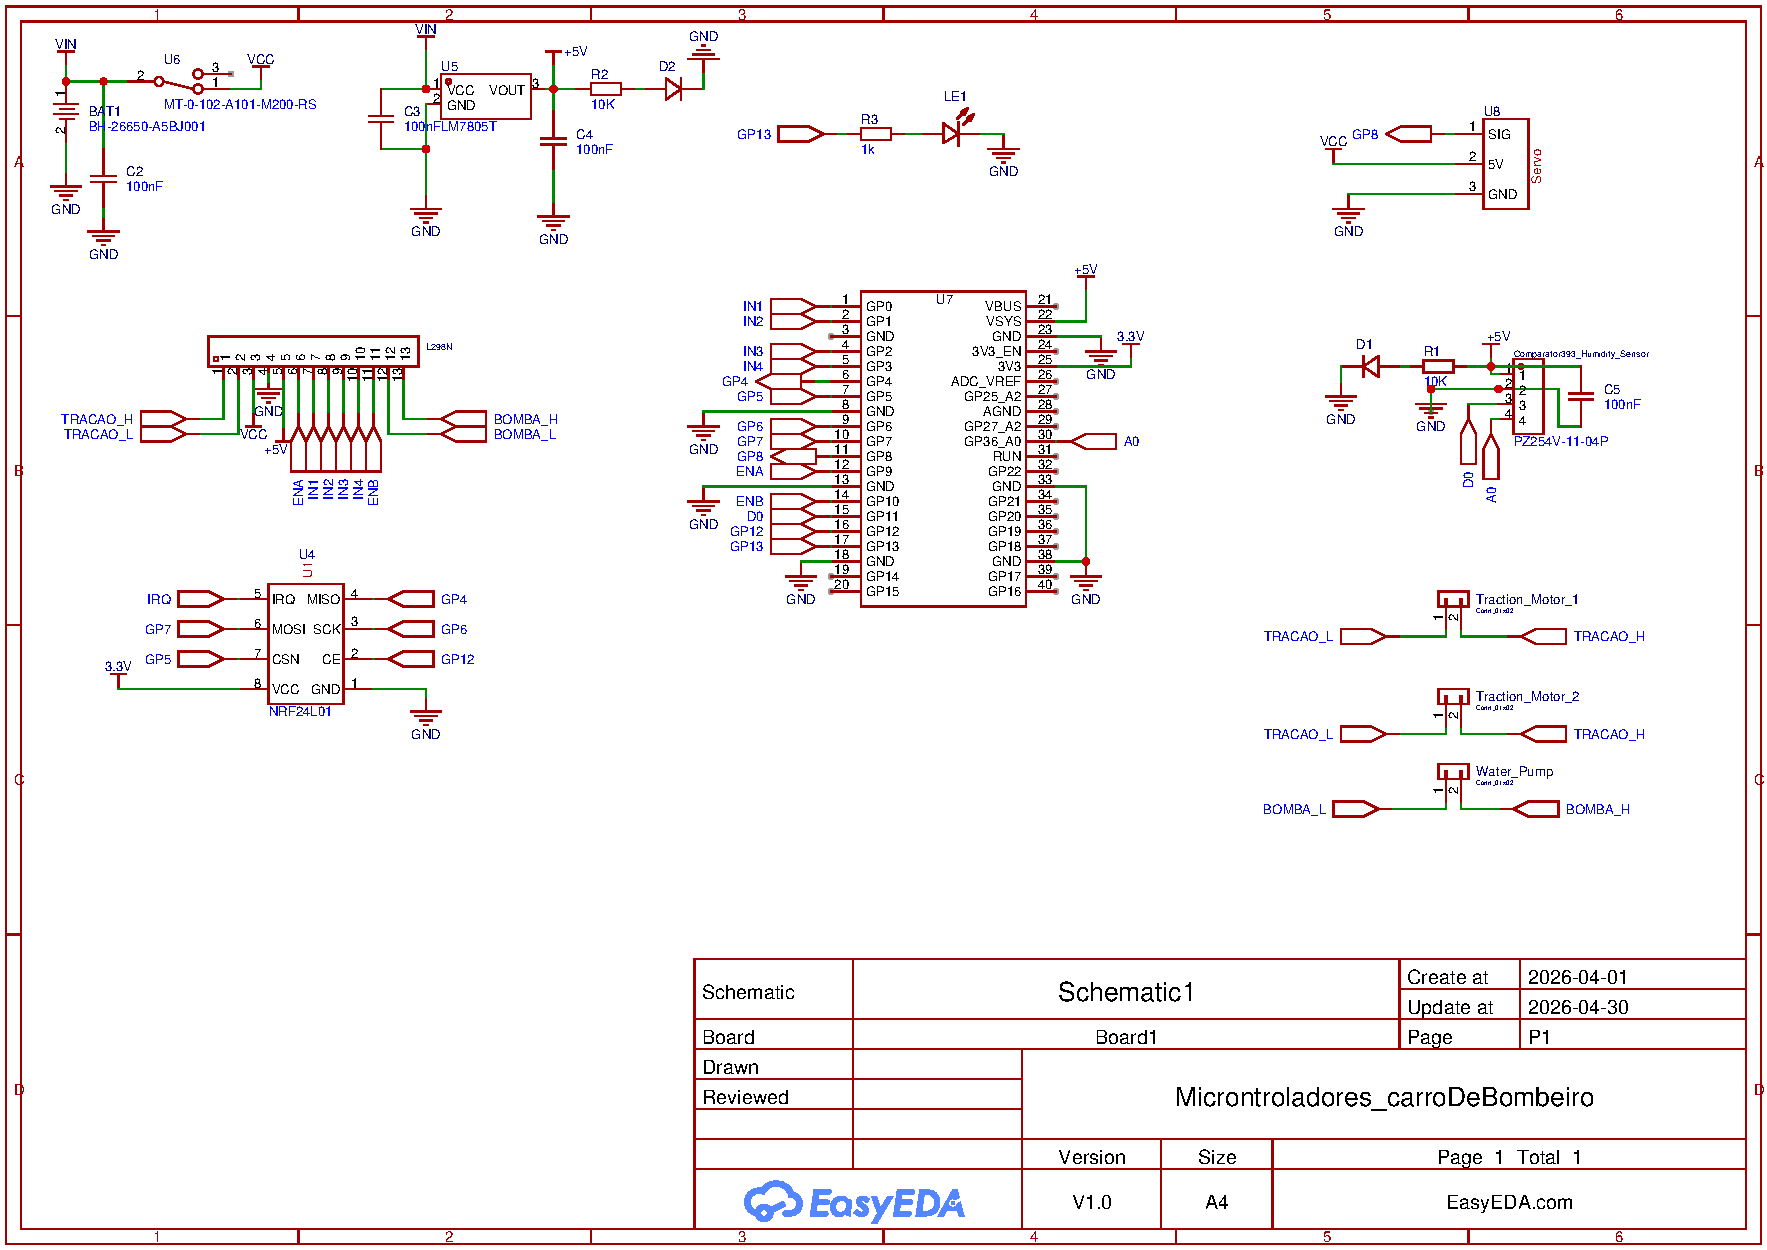
\includepdf[pages=-]{../../Esquemas elétricos/Carro/Esquema elétrico.pdf}

\chapter{Layout da PCB do Carro}
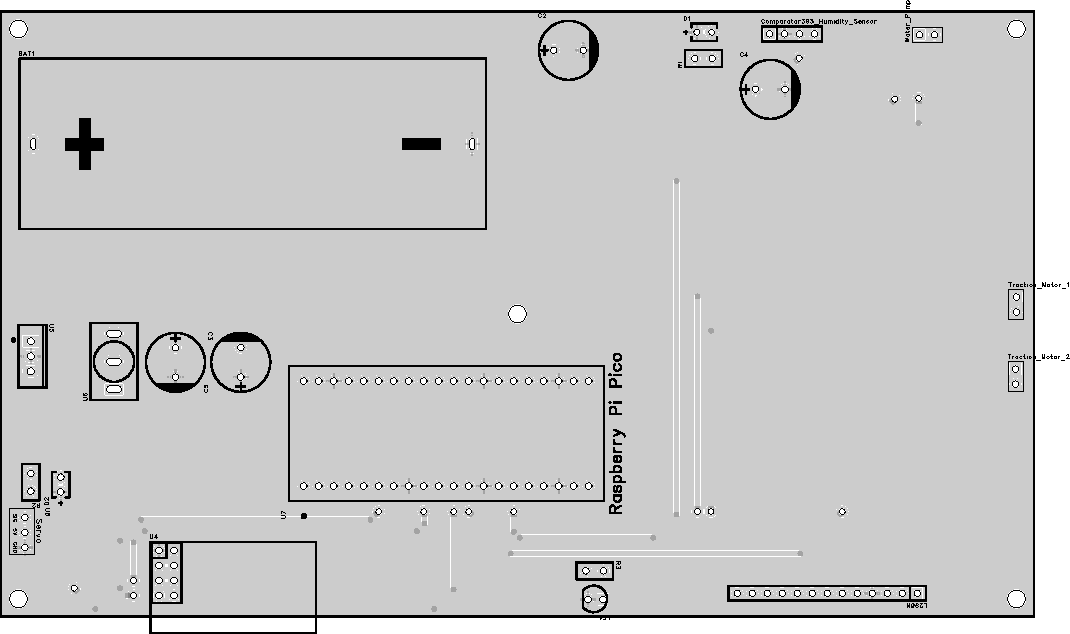
\includepdf[pages=-]{../../Esquemas elétricos/Carro/Esquema PCB.pdf}

\chapter{Esquema Elétrico do Controle}
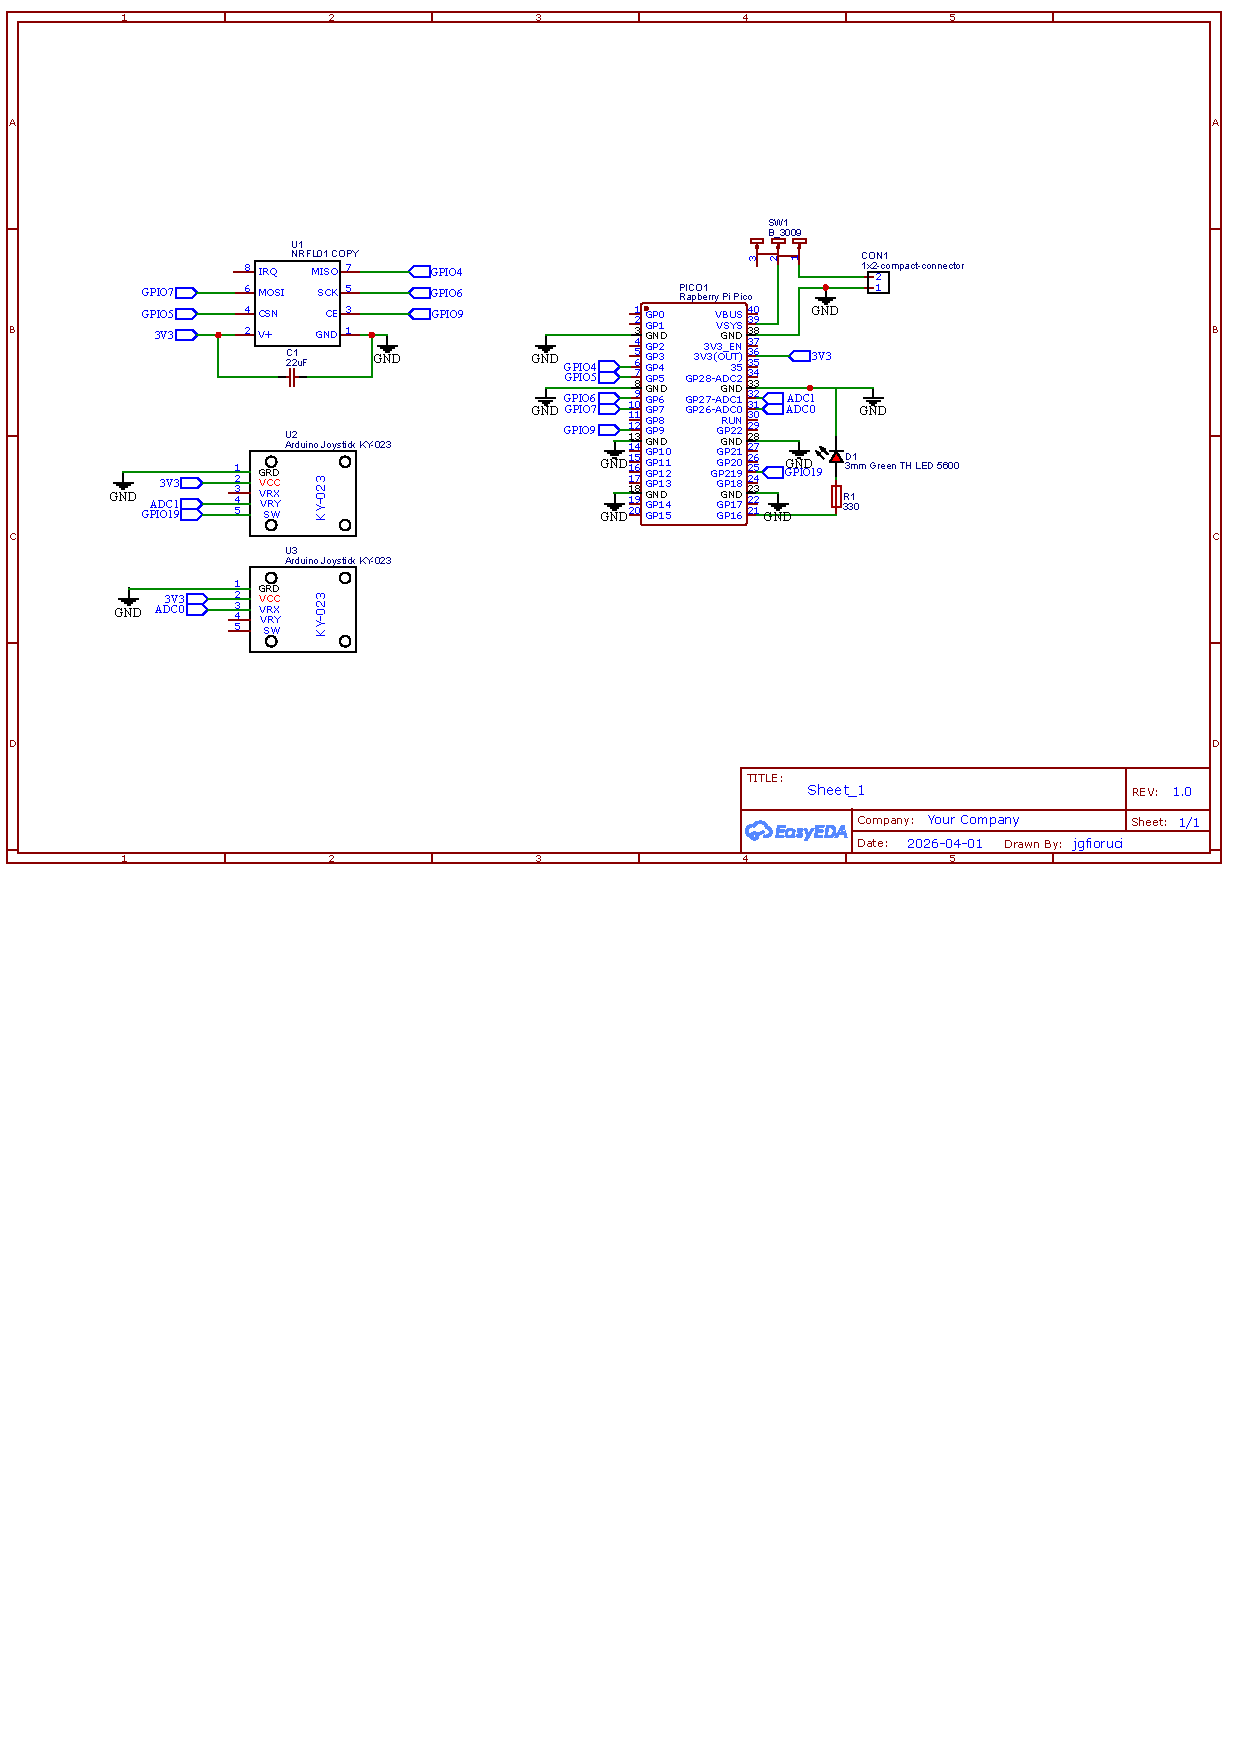
\includepdf[pages=-]{../../Esquemas elétricos/Controle/controle_bombeiro.pdf}

\chapter{Layout da PCB do Controle}
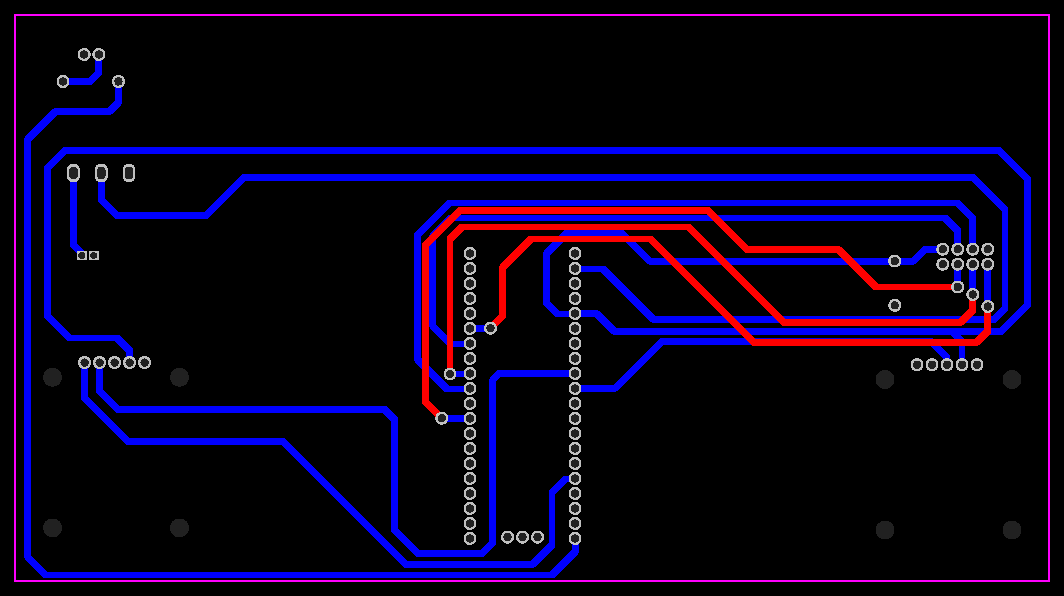
\includepdf[pages=-]{../../Esquemas elétricos/Controle/Esquema PCB.pdf}

\end{anexosenv}

\end{document}
